\documentclass{article}
\usepackage{graphicx}
\usepackage{adjustbox}
\usepackage{float}
\begin{document}

\section{Integration Strategy}
\subsection{Elements to be integrated}
\subsubsection{Client System Strategy}
In order to test the client-related part of our system, we will follow a bottom-up strategy.
First, we will test each functionality-related subsystem, ordering them in this way, from the most critical for the application:
\begin{enumerate}
\item ReservationController
\item BalanceController
\item AccountController
\item RegistrationController
\item ReportController
\end{enumerate}

For each of this subsystem, first we are going to test all the components separatly, then integrate them.
\newline

\textbf{ReservationController}
\\
First we will test the UnlockConditionChecker with the CarActuatorManager Stub and the DatabaseController.
\\
\begin{figure}[H]
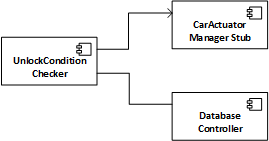
\includegraphics[scale=1]{Images/Reservation/UnlockIntegration.png}
\centering
\end{figure}
Then we will integrate the ReservationTimer with the InfractionManager Stub,
\\
\begin{figure}[H]
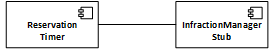
\includegraphics[scale=1]{Images/Reservation/TimerIntegration.png}
\centering
\end{figure} 

followed by the integration between the CarReservator with both DatabaseController and ReservationTimer.
\\
\begin{figure}[H]
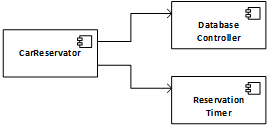
\includegraphics[scale=1]{Images/Reservation/ReservatorIntegration.png}
\centering
\end{figure} 

Lastly we will integrate the AvailableCarRetriever with the DatabaseController. 
\begin{figure}[H]
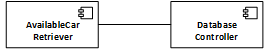
\includegraphics[scale=1]{Images/Reservation/AvailableIntegration.png}
\centering
\end{figure}

At this point we can integrate togheter all the components to test the reservation functionalities.
\begin{figure}[H]
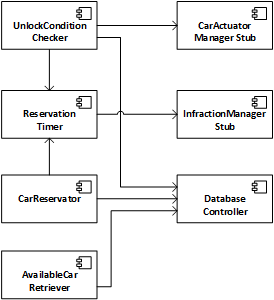
\includegraphics[scale=1]{Images/Reservation/ReservationControllerStrategy.png}
\centering
\end{figure}


\textbf{BalanceController}
\\
First we will integrate the BalanceController with the DataBaseController and the NotificationForwarder. 
\begin{figure}[H]
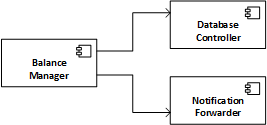
\includegraphics[scale=1]{Images/Balance/ManagerIntegration}
\centering
\end{figure}
Then we will integrate the TransactionProcessor with the PaymentForwarder and the BalanceController.
\begin{figure}[H]
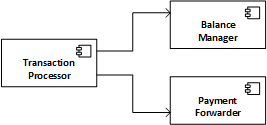
\includegraphics[scale=1]{Images/Balance/TransactionIntegration}
\centering
\end{figure}
In the end we will integrate all the components to test the balance-related functionalities.
\\
\begin{figure}[H]
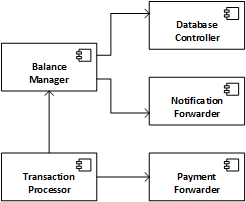
\includegraphics[scale=1]{Images/Balance/BalanceControllerStrategy}
\centering
\end{figure}


\textbf{AccountController}\\
For this subsystem we first integrate the InfractionManager with the BalanceManager and the DatabaseController.

Then we have to integrate the other components with the DatabaseController

\\
\textbf{RegistrationController}\\
For this subsystem we are going to integrate the registration manager first with the DrivingLicenseValidator, then with the PaymentInformationValidator and at last with the DatabaseController

\end{document}

